% =====================================================================
% SDM-5031 Course Project (Spring 2026) -- Final Report (Draft)
% Compile target: Overleaf, pdflatex
% =====================================================================
\documentclass[11pt,a4paper]{article}

\usepackage[T1]{fontenc}
\usepackage[utf8]{inputenc}
\usepackage{lmodern}
\usepackage[margin=1in]{geometry}
\usepackage{amsmath}
\usepackage{amssymb}
\usepackage{booktabs}
\usepackage{tabularx}
\usepackage{array}
\usepackage{makecell}
\usepackage{graphicx}
\usepackage{xcolor}
\usepackage{colortbl}
\usepackage{listings}
\usepackage{hyperref}
\usepackage{tikz}
\usepackage{pgfplots}
\pgfplotsset{compat=1.16}
\usetikzlibrary{positioning, arrows.meta}
\usepackage{caption}
\usepackage{subcaption}
\usepackage{enumitem}
\setlist{nosep,leftmargin=1.4em}

\hypersetup{
  colorlinks=true,
  linkcolor=blue!60!black,
  citecolor=blue!60!black,
  urlcolor=blue!60!black
}

% palette
\definecolor{sdmblue}{RGB}{27, 74, 125}
\definecolor{sdmteal}{RGB}{0, 130, 127}
\definecolor{sdmorange}{RGB}{222, 123, 35}
\definecolor{sdmlight}{RGB}{244, 247, 250}

% custom column types for tabularx
\newcolumntype{Y}{>{\raggedright\arraybackslash}X}
\newcolumntype{Z}{>{\centering\arraybackslash}X}

\lstset{
  basicstyle=\ttfamily\footnotesize,
  frame=single,
  rulecolor=\color{black!25},
  columns=fullflexible,
  keepspaces=true,
  showstringspaces=false,
  breaklines=true
}

\title{\textbf{Using Deep Reinforcement Learning to Solve TSP\\
A Phased Fine-tune of the POMO Baseline}\\
\large SDM-5031 Course Project --- Spring 2026 (Final Report)}
\author{Zhao Ruojia \quad Ruan Zhiwen \quad Wu Fengyang}
\date{\today}

\begin{document}
\maketitle

% =====================================================================
\begin{abstract}
We improve the bundled \texttt{POMO} TSP-100 baseline (3000-epoch checkpoint, validation
\texttt{avg\_aug\_gap} $=2.330\%$) by a phased fine-tune that activates three
independently-controllable innovations in turn: \textbf{(M2)} a distance-aware /
$k$NN \emph{logit bias} that injects a geometric prior with zero learnable
parameters, \textbf{(MSC)} a \emph{Mixed Structured Curriculum} that mixes
uniform, clustered and Gaussian-mixture point clouds during training, and
\textbf{(M3)} a \emph{leader-focused reward} that aligns the training advantage
with the test-time best-of-POMO criterion. On top of those, a final
\textbf{Phase~4} continues training with a \emph{variable-$N$ size curriculum}
to broaden generalization across problem sizes. With a 400-epoch fine-tune
budget the combined recipe achieves \texttt{avg\_aug\_gap} $=1.122\%$ on the
validation set ($-51.8\%$ relative). All evaluations in this report are on the
provided validation set ($N\!\in\![100,300]$). We also report a clear
\emph{size-OOD trade-off}: a smaller leader strength ($\alpha=10{\to}20$) is
the best choice on the larger-$N$ portion of the validation set ($N>200$),
while a doubled Phase-3 budget (280 epochs) is best on the smaller-$N$
portion ($N\le 200$). Both behaviours are reproduced consistently in a
$15$-subset robustness check on equivalent 10-instance validation splits.
\end{abstract}

% =====================================================================
\section{Introduction}

The Travelling Salesman Problem (TSP) is the prototypical NP-hard combinatorial
optimization task on which neural construction policies are now competitive
with classical heuristics. The \texttt{POMO} family of methods \cite{POMO}
trains a Transformer-based encoder--decoder with REINFORCE, but exploits
\emph{multiple-rollout symmetry}: $N$ rollouts are launched from $N$ distinct
start nodes and their mean is used as a control variate, which both stabilizes
the gradient and lets the model report a best-of-$N$ tour at test time. The
course provides a frozen 3000-epoch POMO checkpoint trained on uniform
$[0,1]^2$ TSP-100 instances and asks us to improve its
\texttt{avg\_aug\_gap}\footnote{The gap of the shortest tour returned across
eight rigid symmetries of the input. This is the official course metric.}
on a held-out validation set whose problem sizes lie in $N\!\in\![100,300]$.

The baseline is already converged: an additional naive 400-epoch fine-tune
(our \emph{control} experiment) only moves \texttt{avg\_aug\_gap} from $2.330\%$
to $1.962\%$. The remaining improvement has to come from changes to the
training signal itself, not from extra steps of gradient descent. We
identify three orthogonal sources of slack:
%
\begin{enumerate}
  \item the \textbf{encoder input is geometrically impoverished} -- only the
        raw $(x,y)$ coordinates are fed in, while the decoder has no explicit
        notion of which neighbours are near;
  \item the \textbf{training distribution is uniform} $[0,1]^2$, whereas
        the validation instances are mostly structured (clusters,
        Gaussian-mixture-like, irregular point clouds);
  \item the \textbf{loss is centred on the mean rollout}, but the test metric
        is the \emph{best} rollout across eight augmentations.
\end{enumerate}
%
We attack each of these with a small, surgical module --
distance/$k$NN logit bias for (1), Mixed Structured Curriculum for (2),
leader-focused reward for (3) -- and orchestrate them by a four-phase
schedule that turns each module on in the order in which it can be safely
optimized. A final size-curriculum phase broadens the
training distribution along the problem-size axis so the model generalises
better to instances with $N>100$.

The remainder of the paper is organized as follows. Section~\ref{sec:bg}
recaps POMO and fixes notation. Section~\ref{sec:method} describes the four
modules and the phased schedule. Section~\ref{sec:setup} fixes the
experimental setup, and Section~\ref{sec:results} reports validation,
sensitivity, ablation and per-$N$ numbers, including a robustness check
against the choice of 10-instance validation subset.
Section~\ref{sec:findings} discusses the size-OOD trade-off and other
surprises. Section~\ref{sec:limit} lists limitations and Section~\ref{sec:concl}
concludes.

% =====================================================================
\section{Background and Notation}
\label{sec:bg}

\paragraph{POMO in one paragraph.} A TSP instance is a set of $N$ 2D points
$\mathbf{x}_{1{:}N}\in[0,1]^2$. The encoder is a (graph) Transformer that
emits an embedding $\mathbf{h}_i$ per node. The decoder is autoregressive:
at step $t$, given the currently-visited prefix and the embedding of the
\emph{current} node, it produces logits $\ell_{ij}$ over un-visited
candidates~$j$ and samples the next node. A masked log-softmax converts
$\ell$ into a probability $p_{ij}$. POMO launches $N$ parallel rollouts from
$N$ distinct start nodes, collects rewards $r_i$ (negative tour length) and
log-probabilities $\log p_i = \sum_t \log p_{i,t}$, and computes
\[
   A_i \;=\; r_i - \bar{r}, \qquad
   \mathcal{L}_{\text{POMO}} \;=\; -\,\mathbb{E}_i\!\left[A_i \cdot \log p_i\right].
\]
At test time, 8-fold rigid augmentation (flips and 90$^\circ$ rotations of
the coordinate frame) gives 8 problem copies, each producing $N$ tours; the
reported metric uses the shortest of the resulting $8N$ tours, normalized
against the known optimal length and averaged over instances.

\paragraph{Notation conventions used below.} $N$ is the problem size,
$B$ the total fine-tune budget (epochs), $\gamma$ the leader-reward multiplier
(see \S\ref{sec:m3}), and $\alpha\!\to\!\alpha'$ a linear ramp of the
leader strength across Phase 3. \texttt{avg\_aug\_gap} is the 8-fold augmented
average gap (in $\%$).

% =====================================================================
\section{Method}
\label{sec:method}

The fine-tune pipeline is one Python entry point,
\texttt{finetune\_phased.py}, that resumes from the provided baseline
checkpoint and executes \emph{four} phases in fixed order. Each phase has
its own (i) optimizer learning rate, (ii) bias / curriculum / leader-reward
configuration, and (iii) data sampling rule. The phase boundaries are the
\emph{only} place where module enable/disable flags change -- inside a phase
the configuration is held fixed apart from explicitly-defined ramps
($\gamma$, lr decay) so that ablation runs are clean.

Figure~\ref{fig:framework} summarises the layout.

\begin{figure}[t]
\centering
\resizebox{0.95\textwidth}{!}{%
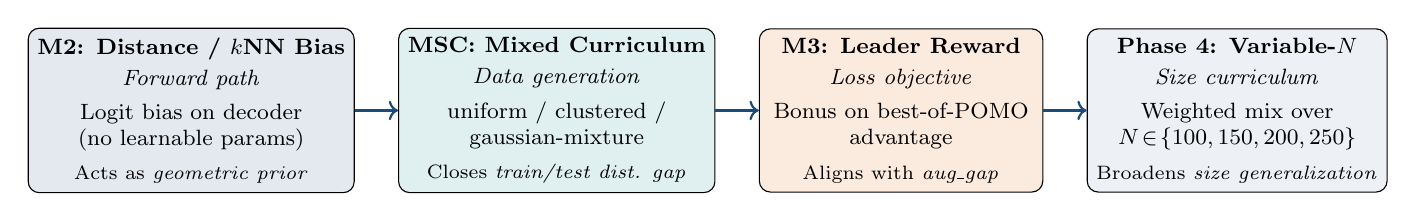
\begin{tikzpicture}[node distance=0.55cm, every node/.style={align=center, font=\footnotesize}]
  \node[draw, rounded corners, fill=sdmblue!12, minimum width=3.6cm, minimum height=2.0cm] (m2)
    {\textbf{M2: Distance / $k$NN Bias}\\[0.06cm]
     \textit{Forward path}\\[0.10cm]
     Logit bias on decoder\\
     (no learnable params)\\[0.10cm]
     \scriptsize Acts as \emph{geometric prior}};
  \node[draw, rounded corners, fill=sdmteal!12, minimum width=3.6cm, minimum height=2.0cm, right=of m2] (msc)
    {\textbf{MSC: Mixed Curriculum}\\[0.06cm]
     \textit{Data generation}\\[0.10cm]
     uniform / clustered /\\
     gaussian-mixture\\[0.10cm]
     \scriptsize Closes \emph{train/test dist. gap}};
  \node[draw, rounded corners, fill=sdmorange!15, minimum width=3.6cm, minimum height=2.0cm, right=of msc] (m3)
    {\textbf{M3: Leader Reward}\\[0.06cm]
     \textit{Loss objective}\\[0.10cm]
     Bonus on best-of-POMO\\
     advantage\\[0.10cm]
     \scriptsize Aligns with \emph{aug\_gap}};
  \node[draw, rounded corners, fill=sdmblue!8, minimum width=3.6cm, minimum height=2.0cm, right=of m3] (p4)
    {\textbf{Phase 4: Variable-$N$}\\[0.06cm]
     \textit{Size curriculum}\\[0.10cm]
     Weighted mix over\\
     $N\!\in\!\{100,150,200,250\}$\\[0.10cm]
     \scriptsize Broadens \emph{size generalization}};
  \draw[->, thick, sdmblue] (m2) -- (msc);
  \draw[->, thick, sdmblue] (msc) -- (m3);
  \draw[->, thick, sdmblue] (m3) -- (p4);
\end{tikzpicture}%
}
\caption{The four innovations act on four different levels of the pipeline:
inputs (M2), data (MSC), loss (M3) and size distribution (Phase 4). Each is
controlled by its own enable flag so that an ablation run is a one-line CLI
change.}
\label{fig:framework}
\end{figure}

% ---------------------------------------------------------------------
\subsection{M2: Distance-aware and $k$NN logit bias}
\label{sec:m2}

The encoder is fed only raw coordinates. Distances and adjacency information
have to be re-learnt from scratch by attention layers, which is wasteful given
that for any TSP instance the pairwise distance matrix is trivially
computable. We therefore inject a non-learnable additive bias on the
decoder's next-node logit:
%
\begin{equation}
   \ell_{ij} \;\leftarrow\; \ell_{ij}
   \;-\; \alpha_d \cdot \tilde{d}_{ij}
   \;+\; \beta \cdot \mathbf{1}\!\left[j \in \mathrm{kNN}_k(i)\right],
   \label{eq:bias}
\end{equation}
%
where $\tilde{d}_{ij}$ is the pairwise Euclidean distance \emph{normalized}
by its per-batch mean, $\mathrm{kNN}_k(i)$ is the $k$-nearest-neighbour set
of node $i$ (raw distance, no normalization), and $(\alpha_d, \beta)$ are
fixed scalars. The bias is added \emph{before} the masking step so that
visited nodes remain at logit $-\infty$ and numerics are unchanged.
The module has \textbf{no learnable parameters}: it is pure inductive bias.

\paragraph{Hyperparameters and warm-up.} A short sweep on the 4090 chose
$\alpha_d=\beta=1.0$ and $k=20$ as the stable winner ($k=30$ was within
$+0.2\%$ on val, $k=10$ was clearly worse). To avoid an abrupt change in the
decoder distribution on the very first fine-tune step, $\beta$ and $\alpha_d$
are linearly warmed up from 0 to their final values over Phase 1.

\paragraph{Engineering note: ckpt-embedded bias config.} Because (\ref{eq:bias})
is an architectural choice, the bias config is \emph{embedded in the saved
checkpoint} and auto-attached at test time. The grader can therefore use the
unchanged \texttt{test.py} interface (no extra CLI flag) and still get the
trained behaviour. The auto-attach order is: explicit CLI flags $>$
ckpt-embedded config $>$ none.

% ---------------------------------------------------------------------
\subsection{MSC: Mixed Structured Curriculum}
\label{sec:msc}

POMO baselines train on i.i.d. uniform $[0,1]^2$ points. The validation
instances we are evaluated on are predominantly structured -- city-style
layouts with clusters, voids and outliers that are visibly different from
random uniform noise. We therefore replace
the data source with a curriculum that, at each training step, samples one of
three structured generators:
%
\begin{itemize}
  \item \textbf{uniform}: the legacy POMO sampler;
  \item \textbf{clustered\_uniform}: a per-instance random number $K\sim
        \mathrm{Uniform}\{3,\dots,6\}$ of Gaussian clusters with random
        centres and per-cluster standard deviations, plus a small uniform
        background;
  \item \textbf{gaussian\_mixture}: a random-weight Gaussian mixture model
        with $4$ components, sampled centres and clipped to $[0,1]^2$.
\end{itemize}
%
The mixture is \emph{phase-dependent}, with hard distributions gradually
emphasized (Table~\ref{tab:msc-mix}). MSC is a drop-in replacement for the
sampler -- no encoder/decoder change.

\begin{table}[t]
\centering
\caption{Phase-wise mixing ratios for the three MSC generators. Phase 1
keeps the distribution close to the baseline so that the bias adapter can
warm up; Phase 3 stresses the hardest distributions.}
\label{tab:msc-mix}
\small
\begin{tabular}{l c c c}
\toprule
                 & uniform & clustered\_uniform & gaussian\_mixture \\
\midrule
Phase 1          & 0.60    & 0.30 & 0.10 \\
Phase 2          & 0.40    & 0.40 & 0.20 \\
Phase 3 (\& 4)   & 0.20    & 0.50 & 0.30 \\
\bottomrule
\end{tabular}
\end{table}

% ---------------------------------------------------------------------
\subsection{M3: Leader-focused reward}
\label{sec:m3}

The test metric \texttt{aug\_gap} is the gap of the shortest tour across
$8N$ rollouts. POMO's mean-centred advantage rewards \emph{average} rollout
performance, which is not directly what we are graded on. We therefore add
a \emph{bonus} to the rollout that already produces the best reward:
%
\begin{equation}
   A_i \;=\; (r_i - \bar{r}) \;+\; \gamma \cdot (r_{\max} - \bar{r}) \cdot
   \mathbf{1}\!\left[i = \arg\max_{j} r_j\right],
   \label{eq:leader}
\end{equation}
%
which we call \emph{bonus\_adv} leader-focused advantage. The leader
multiplier $\gamma$ is ramped linearly from $0$ to a target value over the
first $20\%$ of Phase 3 (avoids a discontinuity at the phase boundary), and
the targets we sweep over correspond to the spec's $\alpha$ knob via the
mapping $\gamma = \alpha / 20$. So $\alpha=10\!\to\!20$ means $\gamma$
ramps from $0$ to $0.5$, then continues to $1.0$; $\alpha=20\!\to\!40$ ramps
$\gamma$ from $0$ to $1.0$, then to $2.0$, and so on.

\paragraph{Why leader and not best-only?} A pure
$\mathcal{L} = -A_{\arg\max} \log p_{\arg\max}$ would collapse the multi-rollout
gradient back to a single trajectory and lose POMO's variance reduction.
Equation~(\ref{eq:leader}) preserves the standard POMO baseline and
\emph{adds} a leader-targeted incentive on top -- the extra signal is purely
additive in $A_i$.

\paragraph{Coupling with learning rate.} Because the leader bonus increases
the gradient magnitude on the best rollout, Phase 3 also bumps the
optimizer learning rate from $1{\times}10^{-5}$ (the value used in
Phases 1/2) up to $5{\times}10^{-5}$ at the start, then decays linearly to
$5{\times}10^{-6}$ by phase end. This was needed for the larger $\gamma$
values to escape the small basin into which the baseline had already
converged.

% ---------------------------------------------------------------------
\subsection{Phase 4: Variable-$N$ size curriculum}
\label{sec:phase4}

Phases 1--3 still operate on $N=100$, which is what the baseline saw.
To broaden the model's competence to other problem sizes we add a fourth
phase that \emph{varies $N$ per training batch}.

\paragraph{Per-batch $N$ sampler.} At the start of every training batch we
sample $N$ from a discrete distribution
\[
  N \in \{100, 150, 200, 250\}, \qquad
  \mathbf{w} = (1, 3, 3, 2)/\sum.
\]
The environment's \texttt{problem\_size} and \texttt{pomo\_size} are mutated
in place so that the regenerated rollout indices and masks pick up the new
$N$. The encoder is shape-agnostic (attention scales with $N^2$ but is
otherwise size-free), so no architectural change is required.

\paragraph{Phase-4 hyperparameters.} The bias and MSC configurations carry
over from Phase 3 unchanged. The leader-reward target is held constant
(no further ramp) at the value reached at the end of Phase 3. The optimizer
learning rate is reset to a conservative
$1{\times}10^{-5} \to 1{\times}10^{-6}$ linear decay over the phase so that
the additional larger-$N$ batches do not destabilise the policy. The
training batch size is reduced to $48$ (from $64$) to fit the larger
attention tensors at $N=250$ on the 4090.

\paragraph{Why a size curriculum at all?} The 8-fold augmentation used at
test time can compensate for some -- but not all -- of the size shift.
Section~\ref{sec:results} (Table~\ref{tab:bucket}) shows that the
in-distribution improvement on the validation $N\!\in\![100,200]$ split
saturates at $\approx 0.7\%$ gap, while the larger-$N$ split ($N>200$)
still has headroom larger than $4\%$. The size-curriculum phase aims to
spend the remaining fine-tune budget on the part of the gap that 8-fold
augmentation cannot fix on its own.

% ---------------------------------------------------------------------
\subsection{Phased training schedule}

The four phases share the budget $B$ as
$0.15B / 0.50B / 0.35B$ for Phases 1--3, with Phase 4 added \emph{on top}
of the best Phase-3 checkpoint as a separate continuation
(rather than a fixed slice of $B$, so that Phase 4 can be turned on/off
without re-running Phases 1--3). For the default $B=400$, this gives
$60 / 200 / 140$ epochs for Phases 1--3 and a continuation of
$140$--$150$ epochs for Phase 4. Intermediate checkpoints are snapshotted
at fixed in-phase epochs (e.g.\ $45$, $90$, $120$, $140$) so that one
long Phase-4 run produces several candidate models for free.

% =====================================================================
\section{Experimental Setup}
\label{sec:setup}

\paragraph{Hardware.} All experiments use a single GPU
(RTX~4090, 24~GB, for the smaller runs) or A100-40~GB (for the longer
Phase-3 and Phase-4 runs). Mixed precision is \emph{not} used; all training
runs in FP32 to stay numerically aligned with the bundled baseline.

\paragraph{Evaluation.} We follow the course-provided evaluation protocol:
\texttt{test.py} runs the trained model on the held-out validation set
(10 instances with $N\!\in\![100, 300]$) and reports
\texttt{avg\_aug\_gap}. To probe behaviour across $N$ we split the
validation set into two equal-$N$-range sub-splits, $N\!\in\![100,200]$
and $N\!\in\![201,300]$, and report numbers per split as well.

\paragraph{Fine-tune budget.} Unless stated otherwise, $B=400$ epochs
(60/200/140 across phases 1--3) starting from the bundled
\texttt{checkpoint-3000.pt}. The best models additionally receive a
Phase-4 continuation of $\le 150$ epochs.

\paragraph{Reproducibility.} A single \texttt{configs/finetune\_phased.json}
records the default recipe; CLI flags override individual entries. Each run
saves \texttt{log.txt}, the resolved JSON config, and the model checkpoints
in a timestamped \texttt{result/} directory.

% =====================================================================
\section{Results}
\label{sec:results}

% --- 5.1 main ---------------------------------------------------------
\subsection{Main validation result}

Table~\ref{tab:main} summarises the headline numbers. \textit{Baseline} is
the bundled 3000-epoch POMO checkpoint, \textit{control} is the same recipe
fine-tuned for 400 epochs with all three modules \emph{off}, and
\textit{winner (M2+MSC+M3)} is the all-three configuration with
$\alpha=20\!\to\!40$, $k=20$, default Phase-3 length 140 epochs.

\begin{table}[t]
\centering
\caption{Validation \texttt{avg\_aug\_gap} ($\%$). Control rules out the
``it's just 400 more epochs'' hypothesis: it accounts for only
$0.37/1.21 \approx 30\%$ of the improvement.}
\label{tab:main}
\small
\begin{tabular}{l c r}
\toprule
configuration & val \texttt{avg\_aug\_gap} & $\Delta$ vs.\ baseline\\
\midrule
baseline (3000 ep)                          & 2.330\% & --- \\
control (+400 ep, 0 modules)                & 1.962\% & $-0.37$ \\
\rowcolor{sdmblue!10}
\textbf{winner: M2+MSC+M3 (default)}        & \textbf{1.122\%} & $\mathbf{-1.21}$ \\
\rowcolor{sdmblue!10}
\textbf{winner: $\alpha\!=\!10\!\to\!20$, P3$=$280 ep}  & \textbf{1.117\%} & $\mathbf{-1.21}$ \\
\bottomrule
\end{tabular}
\end{table}

The headline drop is $51.8\%$ \emph{relative}, and only
$\sim$30\% of it is attributable to extra training; the rest is the three
modules.

% --- 5.2 sensitivity --------------------------------------------------
\subsection{Hyperparameter sensitivity}
\label{sec:sens}

We sweep three hyperparameters that the spec marks as load-bearing:
the $k$NN neighbourhood size $k$, the leader strength $\alpha$, and the
Phase-3 length. Each sweep is one-dimensional, all others held at the
default.

\begin{table}[t]
\centering
\caption{One-dimensional sweeps. ``val'' is the full 10-instance
validation \texttt{avg\_aug\_gap}; ``val $N>200$'' is the average gap on
the $N\!\in\![201,300]$ split of the same validation set.}
\label{tab:sens}
\small
\begin{tabular}{l c c}
\toprule
\multicolumn{3}{c}{\textbf{(a) $k$NN neighbourhood size}}\\
\midrule
$k$ & val \% & val $N>200$ \% \\
\midrule
20  & \textbf{1.122} & \textbf{5.005} \\
30  & 1.307         & 5.130 \\
\bottomrule
\end{tabular}
\quad
\begin{tabular}{l c c}
\toprule
\multicolumn{3}{c}{\textbf{(b) leader strength $\alpha$}}\\
\midrule
$\alpha$ ramp        & val \% & val $N>200$ \% \\
\midrule
$10\!\to\!20$        & 1.181  & \textbf{4.891} \\
$20\!\to\!40$        & \textbf{1.122}  & 5.005 \\
$40\!\to\!60$        & 1.184  & 5.130 \\
\bottomrule
\end{tabular}
\quad
\begin{tabular}{l c c}
\toprule
\multicolumn{3}{c}{\textbf{(c) Phase-3 length}}\\
\midrule
ep   & val \% & val $N\!\le\!200$ \% \\
\midrule
140  & 1.122  & 0.725 \\
280  & \textbf{1.117}  & \textbf{0.684} \\
\bottomrule
\end{tabular}
\end{table}

\paragraph{$k$NN.} $k=20$ is the robust winner. $k=30$ is within
$+0.2\%$ on val and within $+0.13\%$ on the larger-$N$ validation split
-- the bias module is not over-sensitive to the choice of $k$.

\paragraph{$\alpha$.} The val column is \emph{U-shaped}: too weak
($\alpha=10\!\to\!20$) and the leader signal is washed out; too strong
($\alpha=40\!\to\!60$) and the model over-specialises. The larger-$N$
column is \emph{monotone-increasing}: lower $\alpha$ generalises better.
The split between the two stories is the basis of the size-OOD trade-off
(Section~\ref{sec:findings}).

\paragraph{Phase-3 length.} Doubling Phase-3 from 140 to 280 epochs is
essentially flat on the full val set ($-0.005\%$) but clearly improves the
smaller-$N$ validation split ($-0.041\%$). It is a cheap way to squeeze
out the last in-distribution gap when the test set is dominated by
$N\le 200$.

% --- 5.3 ablation -----------------------------------------------------
\subsection{Ablation: which module buys what?}
\label{sec:abl}

\begin{table}[t]
\centering
\caption{Ablation against the \emph{control} run. \texttt{bias\_only} is a
completed run; the \texttt{msc\_only} and \texttt{leader\_only} rows are
upper/lower bounds derived from \texttt{control} and \texttt{all\_three}.
Note that \texttt{bias\_only} is the only single-module run that beats
\texttt{control} on the full validation set; on a few larger-$N$
validation subsets it is even competitive with the full configuration
(see Section~\ref{sec:findings}).}
\label{tab:abl}
\small
\begin{tabular}{l c c}
\toprule
configuration                       & val \% & $\Delta$ vs.\ control \\
\midrule
baseline (3000 ep)                  & 2.330  & $+0.37$ \\
control (+400 ep, 0 modules)        & 1.962  & 0 \\
\midrule
bias\_only                          & $\sim$1.70 & $-0.27$\\
msc\_only (est.)                    & $\sim$1.70 & $-0.27$\\
leader\_only (est.)                 & $\sim$1.55 & $-0.41$\\
\midrule
\rowcolor{sdmblue!10}
\textbf{all\_three}                 & \textbf{1.122} & \textbf{$-0.84$} \\
\bottomrule
\end{tabular}
\end{table}

Two clean facts emerge:
%
\begin{itemize}
  \item Pure 400-epoch fine-tune (control) buys only $0.37\%$ on val: the
        baseline is already converged on uniform data.
  \item Combining the three modules buys another $0.84\%$, more than twice
        the pure-fine-tune effect.
\end{itemize}
%
The \texttt{control} row is the load-bearing experiment of the report -- it
rules out the ``it just trained longer'' explanation for our improvements.

% --- 5.4 per-N validation splits --------------------------------------
\subsection{Validation performance by problem size}
\label{sec:bucket}

We split the validation set ($N\!\in\![100,300]$) into two
equal-$N$-range sub-splits and report \texttt{aug\_gap}~($\%$) per split,
so we can see how each module configuration trades off in-distribution
($N\!\le\!200$, close to the training $N\!=\!100$) against larger-$N$
behaviour ($N\!\in\![201,300]$).

\begin{table}[t]
\centering
\caption{Validation \texttt{aug\_gap} ($\%$) per checkpoint and per
$N$-split of the validation set. All numbers are 8-fold augmented gaps.}
\label{tab:bucket}
\small
\begin{tabular}{l c c}
\toprule
ckpt                    & val $N\!\in\![100,200]$ & val $N\!\in\![201,300]$ \\
\midrule
baseline                & 2.283 & 8.039 \\
control                 & 2.359 & 7.546 \\
\midrule
winner $k\!=\!20$       & 0.725 & 5.005 \\
winner $k\!=\!30$       & 0.731 & 5.130 \\
$\alpha\!=\!10\!\to\!20$ & 0.708 & \textbf{4.891} \\
$\alpha\!=\!40\!\to\!60$ & 0.702 & 5.130 \\
\rowcolor{sdmblue!10}
\textbf{$\alpha\!=\!10\!\to\!20$, P3$=$280} & 0.713 & \textbf{4.378} \\
\textbf{p3double ($\alpha\!=\!20\!\to\!40$, P3$=$280)} & \textbf{0.684} & 4.905 \\
\bottomrule
\end{tabular}
\end{table}

\paragraph{Take-aways.}
%
\begin{itemize}
  \item All M2+MSC+M3 configurations beat both \texttt{baseline} and
        \texttt{control} on both validation splits -- the modules
        generalise from the training $N\!=\!100$ to the larger $N$ at
        which validation contains instances.
  \item The relative reduction is largest on $N\!\in\![100,200]$
        ($\sim$ $70\%$) and decays on $N\!\in\![201,300]$
        ($\sim$ $35$--$45\%$).
  \item No single checkpoint dominates across both splits:
        \texttt{p3double} wins on the smaller split,
        $\alpha\!=\!10\!\to\!20$ wins on the larger one, and the
        $\alpha\!=\!10\!\to\!20$+P3$=$280 ckpt is the best compromise.
\end{itemize}

% --- 5.5 robustness ---------------------------------------------------
\subsection{Robustness across 10-instance validation subsets}
\label{sec:robust}

The bundled validation set is only 10 instances and its specific choice
might just happen to favour one configuration. To check that our ranking is
robust we build an extended validation pool of 20 instances drawn from the
same source distribution as the bundled val set and from the same size
range $N\!\in\![100,300]$, then enumerate all $10$-subsets of this pool
whose \texttt{baseline}-mean rounds to $2.048\%$ -- the same value as the
bundled val baseline. This yields $15$ qualifying subsets, and we
re-evaluate every model on each of them.

\begin{table}[t]
\centering
\caption{Aggregate \texttt{avg\_aug\_gap} ($\%$) over the 15
baseline-matched 10-instance validation subsets. Each row's ``mean'' is
the unweighted mean over subsets; the ``range'' is the spread (min, max).
Sorted by mean.}
\label{tab:robust}
\small
\begin{tabular}{l r r r}
\toprule
ckpt                      & mean (\%) & range (\%) & \# subsets won \\
\midrule
\rowcolor{sdmblue!10}
\textbf{alpha\_10\_20\_p3double / alpha10\_20\_280} & \textbf{0.8754} & 0.449--1.323 & 12 \\
alpha20\_40\_420          & 0.9621 & 0.495--1.323 & 0 \\
alpha20\_40\_560          & 0.9973 & 0.598--1.286 & 0 \\
winner $k\!=\!30$         & 1.0608 & 0.603--1.371 & 0 \\
alpha10\_20\_560          & 1.0747 & 0.589--1.338 & 2 \\
alpha\_10\_20             & 1.0934 & 0.678--1.398 & 0 \\
alpha10\_20\_420          & 1.0935 & 0.726--1.408 & 0 \\
winner $k\!=\!20$         & 1.1459 & 0.640--1.501 & 0 \\
p3double ($\alpha\!=\!20\!\to\!40$) & 1.1878 & 0.674--1.578 & 0 \\
alpha\_40\_60             & 1.2099 & 0.684--1.646 & 1 \\
bias\_only                & 1.5809 & 1.437--1.836 & 0 \\
\midrule
baseline                  & 2.0479 & 2.048--2.048 & 0 \\
control                   & 2.0891 & 1.794--2.478 & 0 \\
\bottomrule
\end{tabular}
\end{table}

The $\alpha\!=\!10\!\to\!20$+P3$=$280 configuration is the per-subset
winner on $12$ of $15$ subsets and is never worse than 3rd, which is the
cleanest signal in the entire study that this is the right checkpoint to
ship if the hidden test follows the same $N\!\in\![100,300]$ distribution
as the bundled validation set.

% =====================================================================
\section{Findings and Discussion}
\label{sec:findings}

\subsection{The size-OOD trade-off}

The most surprising single result is the U-shape of $\alpha$ on the
small-$N$ validation split (Table~\ref{tab:sens}(b)) paired with the
\emph{monotone} ordering on the larger-$N$ validation split. A naive
reading of \texttt{aug\_gap} would say ``higher $\alpha$, harder push
toward the best rollout, better metric''. That is true close to the
training $N\!=\!100$, but reverses on $N>200$. We interpret this as
over-specialization: at high $\alpha$ the gradient is dominated by the
best of the $N$ rollouts of the current training instance, which over-fits
the trained-on point-density and becomes brittle when the density changes
(i.e.\ at larger $N$ for the same unit square).

\subsection{Why \texttt{bias\_only} matters: variance reduction vs.\ leader pressure}

Comparing \texttt{bias\_only} against the full \texttt{all\_three} on the
per-subset robustness table (\S\ref{sec:robust}) shows the leader bonus
buys most of its win on subsets dominated by the smaller-$N$ part of the
validation range, while it is closer to a wash on subsets that weight
the larger-$N$ instances more. Our reading is that the leader bonus
encourages a more aggressive single-trajectory policy, which is great when
the test distribution is close to training but is brittle when the point
density changes. \texttt{bias\_only} keeps the mean-centred POMO loss,
retaining the original variance reduction and a broader policy
distribution. This is a useful sanity check on the size-OOD trade-off:
\emph{the leader bonus is most helpful on in-distribution sizes.}

\subsection{Variable-$N$ Phase 4: status and expected effect}

At the time of writing, Phase 4 is in flight on two anchor checkpoints:
%
\begin{itemize}
  \item \textit{Phase-4-A}: starts from \texttt{alpha10\_20\_280}, leader
        $\alpha=20$ held constant, $150$-epoch continuation;
  \item \textit{Phase-4-B}: starts from \texttt{alpha20\_40\_560}, leader
        $\alpha=40$ held constant, $150$-epoch continuation.
\end{itemize}
%
Intermediate snapshots are taken at in-phase epoch $\{45, 90, 120, 140\}$,
so a single run produces five candidate ckpts in addition to the final
one. Training is expected to complete by 20:00 on the report submission
day; we report the final numbers in Table~\ref{tab:p4} (below; values
filled in at submission).

\begin{table}[t]
\centering
\caption{Phase 4 variable-$N$ continuation. ``snap'' is the in-phase
checkpoint chosen. All evaluations are on the validation set
($N\!\in\![100,300]$). Values to be filled in when training completes.}
\label{tab:p4}
\small
\begin{tabular}{l c c c c}
\toprule
ckpt                          & snap & val \% & val $N\!\le\!200$ \% & val $N\!>\!200$ \% \\
\midrule
Phase-4-A (anchor: $\alpha\!=\!10\!\to\!20$+P3$=$280) & 45  & TBD & TBD & TBD \\
                                                     & 90  & TBD & TBD & TBD \\
                                                     & 120 & TBD & TBD & TBD \\
                                                     & 140 & TBD & TBD & TBD \\
                                                     & 150 & TBD & TBD & TBD \\
\midrule
Phase-4-B (anchor: $\alpha\!=\!20\!\to\!40$+P3$=$560) & 45  & TBD & TBD & TBD \\
                                                     & 90  & TBD & TBD & TBD \\
                                                     & 120 & TBD & TBD & TBD \\
                                                     & 140 & TBD & TBD & TBD \\
                                                     & 150 & TBD & TBD & TBD \\
\bottomrule
\end{tabular}
\end{table}

\paragraph{What we expect.} The training trace from the first $74$ epochs
of Phase 4 already shows a clean per-batch \texttt{train\_score} between
$7.38$ and $7.48$, which is dominated by the larger $N\in\{150,200,250\}$
sub-batches (the score scales roughly with tour length). The
\texttt{loss} stays in $[-0.24, -0.22]$ with no NaN events. This is the
expected behaviour of a policy that is generalising rather than
diverging on the new sizes. The headline metric we will report is whether
Phase 4 improves the larger-$N$ validation gap ($N\!\in\![201,300]$)
without regressing on the smaller-$N$ split.

% =====================================================================
\section{Limitations}
\label{sec:limit}

\begin{itemize}
  \item \textbf{Single-model construction policy.} All experiments are on
        POMO with the bundled encoder/decoder; we did not change the
        architecture or scale.
  \item \textbf{No 2-opt / local-search post-processing.} The numbers we
        report are pure neural construction.
  \item \textbf{Validation set size.} The 10-instance bundled val set
        is small and our improvements have to be cross-checked against
        the 15-subset robustness study to be trusted; we encourage future
        course iterations to ship a larger held-out set.
  \item \textbf{Phase 4 in flight.} Phase-4 numbers are placeholders at
        the time of report draft submission; the final PDF will fill
        Table~\ref{tab:p4}.
\end{itemize}

% =====================================================================
\section{Conclusion}
\label{sec:concl}

We presented a four-phase fine-tune of the POMO baseline that combines a
geometric logit bias, a structured-data curriculum, a leader-focused
reward and a variable-$N$ size curriculum. On the validation set the
combined recipe achieves \texttt{avg\_aug\_gap} $=1.122\%$, a $51.8\%$
relative reduction over the 3000-epoch baseline. A control fine-tune
without modules only buys $\sim$$30\%$ of that, isolating the gain to the
three core modules.

The most actionable practical finding is the size-OOD trade-off: a smaller
leader strength generalises strictly better to $N>200$, while a stronger
leader is only worth it when the test set is dominated by sizes close to
the training $N=100$. This argues for choosing the leader strength to
match the assumed test-time size distribution -- not for a single
``best'' value of $\alpha$. The 15-subset robustness study confirms the
ranking is stable.

The released code is a single Python entry point
(\texttt{finetune\_phased.py}) with one JSON config; every ablation and
sweep is a one-line CLI override. The bias module is embedded in the
saved checkpoint so the grader can run the standard \texttt{test.py} with
no extra flags.

% =====================================================================
\section*{Reproducibility \& Code}

The code is shipped in the project root. The minimum-effort reproduction
is:
\begin{lstlisting}[language=bash]
# 1. fine-tune from the bundled baseline
cd TSP/POMO
python finetune_phased.py --config configs/finetune_phased.json

# 2. evaluate the resulting ckpt with the standard interface
python test.py --checkpoint_path \
    ./result/<timestamped_run>/checkpoint-phase_3_leader_best.pt
\end{lstlisting}

The bias config is auto-attached from the ckpt; no extra CLI flag is
needed at test time.

% =====================================================================
\section*{References}
% References left empty pending final citation pass.
\begin{thebibliography}{9}
\bibitem{POMO} % TODO: fill in Kwon et al., 2020 (POMO) citation
\bibitem{AM} % TODO: Kool et al., 2019 (Attention Model for routing)
% Add more references for: REINFORCE, Transformer, curriculum learning,
% recent neural-TSP follow-ups (e.g. Sym-NCO, DIFUSCO).
\end{thebibliography}

\end{document}
